\chapter{Context Awareness}
\label{ch:context_awareness}

As stated in the introduction, \emph{context awareness} is the term adopted by mobile computing researchers to describe a computer's ability to understand (i.e. be aware of) the situation or context in which it is operating. Of particular emphasis are the \emph{human} context (i.e. the computer \emph{user's} situation) and the \emph{environment} context, but device-specific context can also be important to the extent that it can affect the user (e.g. low battery of the device may affect how the user uses the device and even cause him or her to alter plans based on this situation).

Many definitions of context and context awareness have been proposed, usually reflecting different discipline-specific perspectives. The word context figures prominently in diverse fields including linguistics, psychology, neuroscience, law, and computer science. Due to the great number of definitions, some researchers have used techniques such as \gls{lsa} and \gls{pca} to find the relationships between the many definitions of context \cite{Foltz1998} \cite{Bazire2005}. Others (e.g. \cite{McCarthy1993}) have attempted to formalize the concept mathematically, a topic to which we will turn in Section~\ref{sec:theory}.

Following the approach in \cite{chen_geospatial_2014}, we first present a ``layman's'' definition of context, in order to provide a working, notional notion for our initial discussion. In later sections, we will explore more formal definitions of context. Let us start by seeing how context is defined in a dictionary. In the Merriam-Webster Dictionary, the word context has two definitions \cite{merriam2015}:

\begin{enumerate}
  \item the parts of a discourse that surround a word or passage and can throw light on its meaning
  \item the interrelated conditions in which something exists or occurs : ENVIRONMENT, SETTING
\end{enumerate}

In this thesis, we adopt the second definition. This is because we are not directly concerned with human discourse but rather with conditions of an environment or setting that can be ``understood'' by computers. Clearly, these two definitions are interrelated---discourse is the way that humans articulate their understanding of an environment or setting. Put in another way, natural language is how humans encode contextual information. In this thesis, we focus on techniques that computers can use to represent and process context without human intervention. When we refer to context, we refer directly to the conditions in the environment rather than representations of context, such as discourse. As noted in Section~\ref{sec:objectives}, \emph{situation} can be used as a synonym for context. We see no reason to distinguish between the two terms, although we note that some formalisms make a distinction (see \cite{akman1996steps}).

With this working definition of context established, we proceed to the remainder of the chapter, which is organized as follows. First, we provide a simple framework for specifying a context (i.e. the ``interrelated conditions'') in Section~\ref{sec:framework}. Then, in Section~\ref{sec:history} we present a brief historical overview of context awareness, which also serves as a review of the early context awareness literature. Next, Section~\ref{sec:literature} provides a review of more recent context awareness literature, paying particular attention to studies relevant to the three tasks described earlier in Section~\ref{sec:objectives}. Section~\ref{sec:theory} presents context in a more formalized manner, using one of the dominant formalizations found in the literature, the \gls{plc}. In this section, we also discuss the differences between \gls{plc} and the notion of context described above. Finally, Section~\ref{sec:how} describes the sources and methods of context awareness.

\section{A Framework for Contextual Information}
\label{sec:framework}

Because context is such an abstract concept, it is useful to choose some techniques for describing a particular context. These techniques can be used to build a framework for expressing contextual information. The goal of this section is to describe one such technique. We make no claim that this technique or framework is an authoritative one, nor that it is complete in the sense of exhaustively covering the concept of context.

In our view, the goal of context-aware systems is essentially to mimic the way that humans understand and describe situations, contexts, conditions, or events (we use all these terms almost interchangeably, although they may emphasize different aspects, such as fixed versus dynamic elements). According to this goal, we might employ the classic technique of journalism (since journalism is an age-old craft for describing conditions and events), known as the \acrshort{fiveWs}: \acrlong{fiveWs} \ci{wiki2015}. This technique can be traced back to the late 2nd century \acrshort{bc} when Hermagoras of Temnos defined seven elements of circumstance, which includes (in addition to the Five Ws) ``in what manner'' and ``by what means'' \cite{bennett2005hermagoras}.

Using these questions as a framework (with a slightly different order), the following provides an example of elements of a particular context:
%
\begin{bold_description}
\item[What:]A small gathering of colleagues for lunch
\item[Who:] Present are Mary, Philip, George, and Anita
\item[Where:]60.1609\textdegree{}\acrshort{n}, 24.5460\textdegree{}\acrshort{e} (\acrshort{wgs84}); inside the lunch-room of the Finnish Geospatial Research Institute (FGI) in Masala, Finland
\item[When:]Tuesday, 10 March 2015 at 11:03AM
\item[Why:]Because it is lunchtime, and it is the custom for this group of colleagues to eat lunch together.
\item[In What Manner:] Mary's smartphone is experiencing small, sporadic movements, but it mostly remains in a constant orientation. Mary's smartwatch is experiencing more dramatic but also sporadic movements. Both sources of motion data are consistent with a user who is sitting and having a casual conversation and/or eating lunch. Multiple human voices are engaged in conversation of an informal and lively manner.
\item[By What Means:]All of the above information has been sensed or reasoned by the sensors and software existing in a smartphone and a smartwatch, plus some additional sensor data recorded by a networked node installed in the lunch-room. In this case, the smartphone is a Samsung Galaxy S5 with Android 4.4.2 \gls{os}, which includes a \gls{gps} receiver, \acrshort{wlan}-based positioning engine, Bluetooth connectivity, microphone and audio analyzer, ambient light sensor, accelerometers, gyroscopes, compass, and magnetometers. The smartwatch is an LG G Watch with accelerometers, gyroscopes, Bluetooth connectivity, microphone, and an audio analyzer. It runs Android Wear 5.0.1.
\end{bold_description}

This depiction of the situation is not likely to win a Pulitzer Prize in Journalism, probably because the situation is not particularly interesting. Also, note that it has not been formulated completely into prose but rather is more like a set of notes that a journalist might jot down for later use (except maybe for the latitude and longitude coordinates and the motion description). The ``By What Means'' section can also be thought of as notes as to the ``source'' that the journalist might record along with the other information (especially if the account is second-hand).

The following provides an introduction to the context framework proposed in this thesis:
%
\begin{itemize}
\item ``What'' usually refers to the \emph{activity context}, that is, what is actually happening. In some contexts, there might be little ``action'' taking place, but it may also be of interest for some purposes that ``nothing is happening''.
% 
\item ``Who'' refers to the human characters in the context. When speaking about context-aware mobile devices, the user of the mobile device in question is usually the main character, whereas others in the environment can be thought of as supporting characters. The ``who'' portion can also be summarized as the \emph{user and social context}. 
%
\item ``Where'' refers to the \emph{location context}. The most important point to note is that location can be expressed in many different ways: geographic coordinates, an address, or some semantic representation such as ``the Finnish Geospatial Research Institute'' or perhaps more personalized, such as ``my workplace''.
%
\item ``When'' is the \emph{time} and \emph{date context}. We need only to be careful about specifying things like time zones. In addition, it may be important to encode some common sense or semantic knowledge about meaningful aspects, such as ``this is after work hours'' or ``today is a holiday''. Time can be specified either as a specific moment, such as in the example above, or as a time or date segment (e.g. 10--20 March 2015).
%
\item ``Why'' can be thought of as the \emph{motivational context}, e.g. Why is the user doing that? Why is this event taking place?, etc. It could also be appropriate to encode information about whether the context is normal or unusual, as well as an explanation for the unusual events. For example, if a person normally commutes to work along $route A$, and in the present he or she is driving along $route B$, then ``why'' would be a good place to capture the fact that ``there was an accident along $route A$, so the alternate $route B$ was chosen''.
%
\item ``In What Manner'' is a bit of a ``catch all'' category. It is used to provide additional details that do not fit nicely into any of the other categories. This is less than ideal for any formal system of context, but rather than attempting to list out all the possible categories of context (which is probably impossible), we believe it is more practical to have an ``other'' category. One way that we use this category is to capture the \emph{motion context}. This is similar to the activity context, but it is more focused on detailed attributes of the motion. For example, if the current activity of a user is ``dancing'', then ``in what manner'' might be used to capture the type of dance and the tempo in which the user is dancing.
%
\item ``By What Means'', as mentioned above, is to capture the source of the contextual information. It includes information about the devices and sensors used in the context-aware system, as well as the reasoning methods employed.
\end{itemize}

Further details about this framework are covered in [P1]. As context-aware systems develop, we suspect that our framework may change slightly. It is difficult to anticipate what types of contextual information will become important in the future, but this framework should be broad enough to encompass most types of contextual information. Also, our intention is not to have a rigid framework that constrains all future context-aware systems, but rather it is to provide a rough skeleton upon which to experiment and build more elaborate and detailed context ontologies.

\section{History}
\label{sec:history}

According to our review of the literature, the first explicit reference to context awareness was in a 1994 paper by Schilit and Theimer, where they use the term \emph{context-aware computing} to describe software that can ``adapt according to its location of use, the collection of nearby people and objects, as well as the changes to those objects over time.'' \cite{schilit1994disseminating}. Earlier, however, we can find strong but implicit references to the concept of context awareness. For example, in the 1991 article, titled ``The Computer for the 21st Century,'' Weiser provides a fictional account of a number of different automated or computer-assisted functions made possible by ``ubiquitous computing'' \cite{weiser1991computer}. Although not specifically highlighted by Weiser, the necessity of these computers to understand context is clearly evident. Another article, published in 1992 by Want et al., may be the first implementation of a context-aware device described in the literature, even though the authors did not use the term ``context-aware'' \cite{want1992active}. By the mid-1990s, many different implementations of context-aware devices can be found, including the ParcTab, stick-e notes, CyberGuide, and CyberDesk. By 2001, the research field was active enough to support a special issue of the journal \gls{hci}, which provides an excellent review of the state-of-the-art in context awareness for that time period \cite{moran2001introduction}.

Going further back, however, the concept of context has been studied in computer science research for many years. As early as 1963, John McCarthy, one of the ``fathers of AI'', began developing \emph{situation calculus} as a ``formal system in which facts about situations, goals and actions can be expressed'' \cite{mccarthy1963programs}. A situation is defined as ``the complete state of affairs at some instant of time'', thus, it is roughly equivalent to our definition of context. Beginning in 1987, McCarthy began to consider the concept of context explicitly and attempted to formalize it. This work on context and related theory will be presented in Section~\ref{sec:theory} below.

Formalisms of context, however, do not appear to have led directly to the realization of any context-aware software or devices, except for perhaps one example, Cyc, which will discussed further in Section~\ref{sec:theory}. The context-aware devices and applications of the 1990s mostly consisted of location-aware devices, and in our opinion, they do not require an elaborate formalism of context. Nonetheless, the work of McCarthy and others pioneers who offered formalisms of context are worthy of mention in the history of context awareness. In particular, we refer the interested reader to \cite{McCarthy1993} \cite{guha1991contexts} \cite{mccarthy1997formalizing} \cite{akman1996steps}, and \cite{buvac1993propositional}. In addition, \cite{brezillon1999context} and \cite{akman2002context} provide excellent reviews of context in artificial intelligence.

\section{Related Studies}
\label{sec:literature}

A comprehensive review of recent context awareness literature would require covering hundreds, if not thousands, of different studies. The review found in \cite{Hong2009}, which only looks at journal articles published between 2000 and 2007, covered well over 200 different studies.  Searches of several major databases of scientific publications (e.g. IEEE Xplore Digital Library, ACM Digital Library, SpringerLink) using the keyword ``context-aware'' each yielded thousands of results. Clearly, these publications will vary greatly in their relevance to this thesis. To help focus on only the most relevant literature, we only include publications related to the three context awareness tasks described in Section~\ref{sec:objectives}, divided into respective sub-sections below.

\subsection{Context Awareness for Office Environments}
\label{sec:office-literature}

%\hl{
In terms of the first task, recognizing the activity of a smartphone user in an indoor office environment, there are only a few studies basing their results on smartphone sensors, and they mainly rely on location awareness. For example, one early study described user tests of a context-aware \gls{pda} application, which can be considered a proto-smartphone-like mobile device, designed to be used in an office environment \cite{Tahti2004}. The main source of contextual information was location, but the application also used contextual information from calendar events that the user had previously recorded in the application. For example, if a user scheduled an event at a particular time and marked it as a meeting, then the system would automatically suggest meeting-related services when the meeting time approached and the user had entered the meeting room. The described system, however, was not capable of automatically inferring office activities independently from user-supplied information.

More recently, \cite{heiskala2014research} described a pilot study related to smartphone-based context awareness of ``mobile knowledge work'', which may partly take place in office environments. The article, however, mainly discusses the research problem in general, as well as describing the pilot data collection campaign. The article does not go into any detail on the results of analyzing the collected data, nor the planned analysis methods.

If we include studies using non-smartphone sensors to detect office-related activities, we encounter several other relevant studies. For example, \cite{huang2004office} %OFFICE PRESENCE DETECTION USING MULTIMODAL CONTEXT INFORMATION
used a microphone and a USB %acronym
camera to detect different office activities and motion patterns, including ``rest,'' ``moving near door,'' ``conversation,'' ``nobody around,'' etc. They used two machine learning techniques to detect motion and activity: Incremental Hierarchical Discriminant Regression (IHDR) trees and Hidden Markov Models (HMM). \cite{danninger2008context} similarly used a set of cameras to detect whether an office worker is working alone or in a meeting, or whether the office is empty. For activity detection, they used adaptive background modeling, which makes use of Gaussian mixture densities \cite{stauffer1999adaptive}.

Another example is \cite{manabe2010perceptual}, which used a richer set of sensors, including two USB cameras, a pressure sensor, and an acceleration sensor (a Wii remote controller) built into an office chair. This study focused on detecting location and posture context, such as leaning back in the chair, leaning on the desk, or upright sitting posture. They primarily used k-means and \gls{knn} %acronym
clustering to perform context recognition. Similarly, \cite{kiyokawa2012owens} % Owens Luis - A Context-aware Multi-modal Smart Office Chair in an Ambient Environment
presented a so-called ``smart office chair'' designed to measure an office worker's mental and physiological states, such as sleepiness and concentration. The details of the recognition algorithm, however, are not given in the paper.

One study used a combination of mobile phone sensors and room occupancy sensors installed in an office environment \cite{rachuri2014smartphone}. The resulting application, called \emph{WorkSense}, was able to detect when and where meetings and conversations took place. By sensing social interactions, the authors were also able to identify project groups automatically.

Other relevant studies have focused on using wearable sensors to detect different activities, some of which are common in office environments. For example, \cite{kern2003multi} % Multi-sensor Activity Context Detection for Wearable Computing.
used accelerometers attached to various parts of a person's body. Although they did not specifically focus on an office environment, some of the activities they addressed are very relevant. These include sitting, standing, walking, writing on a whiteboard, typing on a keyboard, and shaking hands. The authors used a na\"{i}ve Bayes classifier for activity recognition. Similarly, \cite{pirttikangas2006feature} used wearable sensors to detect several different office-related activities (typing, cleaning a whiteboard, using an elevator, etc.). The authors evaluated the use of \gls{knn} and \gls{mlp} classifiers for activity recognition\footnote{MLP is a type of \gls{ann}.}.


% Mobile phones play a pivotal role in supporting ubiquitous and unobtrusive sensing of
% human activities. However, maintaining a highly accurate record of a user’s behavior
% throughout the day imposes significant energy demands on the phone’s battery. In this
% work, we investigate a new approach that can lead to significant energy savings for
% mobile applications that require continuous sensing of social activities. This is achieved by
% opportunistically offloading sensing to sensors embedded in the environment, leveraging
% sensing that may be available in typical modern buildings (e.g., room occupancy sensors,
% RFID access control systems).
% In this article, we present the design, implementation, and evaluation of METIS: an
% adaptive mobile sensing platform that efficiently supports social sensing applications. The
% platform implements a novel sensor task distribution scheme that dynamically decides
% whether to perform sensing on the phone or in the infrastructure, considering the energy
% consumption, accuracy, and mobility patterns of the user. By comparing the sensing
% distribution scheme with sensing performed solely on the phone or exclusively on the fixed
% remote sensors, we show, through benchmarks using real traces, that the opportunistic
% sensing distribution achieves over 60% and 40% energy savings, respectively. This is
% confirmed through a real world deployment in an office environment for over a month: we
% developed a social application over our frameworks, that is able to infer the collaborations
% and meetings of the users. In this setting the system preserves over 35% more battery life
% over pure phone sensing.


Finally, \cite{Park2015} % ReLiSCE: Utilizing Resource-Limited Sensors for Office Activity Context Extraction
studied context recognition in a meeting room environment, using a suite of sensors including: a microphone array, passive infrared sensors, and an illumination (light) sensor. They detected different states of activity in the meeting room, such as: presentation, monologue, discussion, room idle, people entering room, and room in use. They do not describe their context recognition algorithm in any great detail, but it appears to be a heuristically-defined rule-based algorithm.

The relatively small number of studies related to context awareness in an office environment suggests this is a fairly immature research topic. We can conclude from our literature review that the research in this thesis is rather novel, especially with regards to smartphone-based context awareness for office environments.
%
\subsection{Context Awareness for Mobility}
\label{sec:mobility-context-literature}

With regards to the second task, recognizing modes of motion that a smartphone user is undergoing outdoors, there are comparatively many relevant studies. Despite this fact, to our knowledge no systematic review of this research area has been published, but a few related reviews are available. For example, \cite{Duncan2009} reviews literature on the use of GPS to study health-related physical activity. The focus of this review, however, is mostly on assessing health behavior, rather than on methods to detect different mobility contexts.  \cite{hoseini2013survey} reviews smartphone-based ``opportunistic user context recognition'', which includes some literature on mobility context recognition, and similarly \cite{pejovic2015anticipatory} reviews ``anticipatory mobile computing''. While useful in our review of the literature, none of these reviews focus specifically on mobility context awareness, and they exhibit significant gaps in this regard.

Due to the large number of relevant studies, we will not describe them individually, but pertinent facts from these studies can be found in Table~2.1. We make no claim that this compilation of publications on the subject is exhaustive, but it is, according to our knowledge, the most comprehensive compared to existing literature. We decided to include also studies that utilized wearable sensor modules, since this research is closely linked to smartphone-based research. All of the listed studies used supervised machine learning techniques, except for \cite{kwon2014unsupervised}, which evaluated several different unsupervised learning techniques.

Note also that many of the studies investigate not solely mobility contexts but also other contexts, such as \gls{adl} or various posture contexts (sitting, lying down, etc.). In Table~2.1, we have only identified the relevant motion-related modes. Some other motion-related contexts, such as using an elevator or walking upstairs/downstairs, were investigated by a few studies, but we listed only those modes common to a significant number of studies. For those studies incorporating additional contexts, we have identified these contexts collectively using the symbol ``+''. Lastly, we point out that some of the included studies investigated indoor motion modes, even though our research task was to study outdoor mobility contexts. 

\setlength{\LTcapwidth}{\linewidth}
\begin{center}
\label{tab:literature}
\begin{longtable} {|l|>{\raggedright}p{3cm}|p{2.4cm}|>{\centering\arraybackslash}p{2.5cm}|>{\centering\arraybackslash}p{2.2cm}|}
\caption[Publications related to mobility context]{Publications related to mobility context. The definitions for the abbreviations used for algorithms/techniques are given in the Abbreviations section provided above. The abbreviations used for the motion modes are as follows: S = static (including standing, sitting, etc.), W = walking, R = running/jogging, B = riding a bicycle, D = driving a motor vehicle, MT = any kind of motorized transport (including car, bus, train, etc.), RB = riding a bus, RT = riding a train/tram/light-rail, and RS = riding a subway/metro. ``+'' indicates that other motion modes are also covered by the publication.} \\
\hline \multicolumn{1}{|c|}{\textbf{Year}} & \multicolumn{1}{l|}{\textbf{Author(s) \& Citation}} & \multicolumn{1}{c|}{\textbf{Device(s) Used}} & \multicolumn{1}{>{\centering\arraybackslash}p{2.5cm}|}{\textbf{Algorithm(s) / Technique(s) Evaluated}} & \multicolumn{1}{>{\centering\arraybackslash}p{2.2cm}|}{\textbf{Motion Modes Studied}} \\ \hline 
\endfirsthead
%\begin{tabular}{@{}|l|>{\raggedright}m{3cm}|>{\raggedright}m{2.5cm}|m{2cm}|m{3cm}|>{\raggedright}m{1.5cm}@{}} 

\multicolumn{3}{c}%
{{\bfseries \tablename\ \thetable{} -- continued from previous page}} \\
\hline
\multicolumn{1}{|c|}{\textbf{Year}} & \multicolumn{1}{l|}{\textbf{Author(s) \& Citation}} & \multicolumn{1}{c|}{\textbf{Device(s) Used}} & 
  \multicolumn{1}{>{\centering\arraybackslash}p{2.5cm}|}{\textbf{Algorithm(s) / Technique(s) Evaluated}} & \multicolumn{1}{>{\centering\arraybackslash}p{2.2cm}|}{\textbf{Motion Modes Studied}} \\ \hline 
\endhead

%\textbf{Year} & \textbf{Author(s)} & \textbf{Device(s) Used} & \textbf{Algorithms Evaluated} & \textbf{Motion Modes Studied}\\ \hline
2000 & Foerster, Smeja \& Fahrenberg \cite{foerster2000motion} & accelerometers & rule-based & S, W, B, + \\ \hline
2002 & Lee \& Mase \cite{lee2002activity} & sensor module & fuzzy-rule-based & S, W, + \\ \hline
2005 & Lester et al. \cite{lester2005hybrid} & sensor module & AdaBoost, NB & S, W, R, B, + \\ \hline
2005 & Ravi et al. \cite{Ravi2005} & sensor module & DT, kNN, SVM, NB, meta-classifiers& S, W, R\\ \hline
2006 & P\"{a}rkk\"{a} et al. \cite{parkka2006activity} & various sensors & rule-based, DT, ANN & S, W, R, B, RB, + \\ \hline
2006 & Pirttikangas, Fujinami, \& Nakajima \cite{pirttikangas2006feature} & sensor modules & ANN, kNN & S, W, R, B, + \\ \hline
2007 & Suutala, Pirttikangas \& R\"{o}ning \cite{Suutula2007} & sensor modules & SVM, HMM, SVM-HMM, DTS & S, W, R, B, + \\ \hline
2008 & Kunze \& Lukowicz \cite{kunze2008dealing} & sensor modules & DT, kNN, BN & S, W, R, B, + \\ \hline
2008 & Jin et al. \cite{yin2008sensor} & sensor modules & fuzzy-rule-based & S, W, R, + \\ \hline
2009 & Yang \cite{yang2009toward} & mobile phone & DT, NB, kNN, SVM, HMM & S, W, R, B, D, + \\ \hline
2010 & Reddy et al. \cite{Reddy2010} & mobile phone & DT, KMC, NB, ANN, SVM, CHMM, DT+DHMM & S, W, R, B, MT,  \\ \hline 
2010 & Pei et al. \cite{Pei2010} & mobile phone & rule-based &  S, W, + \\ \hline
2010 & Frank et al. \cite{Frank2010}& sensor module & NB, BN, HMM & S, W, R, + \\ \hline
2011 & Stenneth et al. \cite{Stenneth2011}& mobile phone  & DT, NB, BN, RF, ANN & S, W, B, D, RB, RT \\ \hline
2011 & Pei et al. \cite{pei2011using} & mobile phone & DT, BN, SVM & S, W, + \\ \hline
2011 & Susi, Borio, \& Lachapelle \cite{susi2011accelerometer} & sensor module & DT, NB, kNN & S, W, R, +\\ \hline
2012 & Bancroft et al. \cite{Bancroft2012}& sensor modules & NB, rule-based & S, W, R, B, MT, +\\ \hline
2012 & Anguita et al. \cite{anguita2012human} & mobile phone & SVM, HF-SVM & S, W, + \\ \hline
2013 & Guinness \cite{Guinness2013}& mobile phone & 20 different algorithms & S, W, R, D, RB, RT, +\\ \hline
2013 & Susi, Renaudin, \& Lachapelle \cite{susi2013motion}& sensor modules & DT & S, W, + \\ \hline
2013 & Feng \& Timmermans \cite{feng2013transportation}& sensor module  & BN & W, R, B, D, RB, RT \\ \hline
2013 & Hemminki, Nurmi \& Tarkoma \cite{hemminki2013accelerometer}& mobile phone & HMM, Adaboost, meta classifier & S, W, RB, RT, RS \\ \hline
2014 & Stenneth \cite{stenneth2014detecting} & mobile phone & NB, BN, DT, RF, ANN, meta-classifiers & S, W, B, D, RB, RT\\ \hline
2014 & Xia et al. \cite{xia2014using}& mobile phone & SVM & S, W, B, D\\ \hline
2014 & Elhoushi et al. \cite{elhoushi2014robust}& mobile phone & DT & W, R, B, MT \\ \hline
2014 & Parvainen et al. \cite{parviainen2014adaptive} & mobile phone & DT, SVM, MAP & S, W, R, B, MT \\ \hline
2014 & Yu et al. \cite{yu2014big} & sensor module + mobile phone & DT, AdaBoost, SVM & S, W, R, B, MT \\ \hline
2014 & Kwon, Kang, \& Bae \cite{kwon2014unsupervised} & mobile phone & GMM, kMC, HIER, DBSCAN & S, W, R, +\\ \hline
2014 & Sankaran et al. \cite{sankaran2014using} & mobile phone & rule-based, GPSAR, FMS & S, W, MT \\ \hline
2014 & Chiang, Yang \& Tu \cite{chiang2014pattern} & mobile phone & DT, NN, NB, SVM & S, W, R, B, D, + \\ \hline 
2015 & Yu and Cho \cite{yu2015low} & mobile phone & DT, SVM, ANN & S, W, R, D, RB, RT, RS \\ \hline
\end{longtable}
\end{center}
%
%(Suutula et al., 2007): Activities of daily living
% Discriminative Temporal Smoothing for Activity Recognition from Wearable Sensors
%
%(Heiskala et al., 2014) % Doesn't describe actual context recognition, just data collection system
% A Research Framework for the Smartphone-Based Contextual Study of Mobile Knowledge Work 
%
% (Rasekh et al., 2011) % Maybe use...
%Human Activity Recognition using Smartphone
%
%(Adams et al., 2008)  % PRINT THIS
% Sensing and Using Social Context
%
%(Schuster et al., 2013) % Taxonomy of social context
% Pervasive Social Context: Taxonomy and Survey
%
%(Do and Gatica-Perez, 2013) % Bluetooth-based social context detection
% Human interaction discovery in smartphone proximity networks
%
% Where and what: Using smartphones to predict next locations and applications in daily life
%
%Soikkeli et al., 2014) % Framework/ontology
%Context Classification Framework for Handset-based End User Studies
%
\subsection{Ice Awareness for Maritime Navigation}
\label{sec:ice-awareness-literature}

Regarding the third task, determining the optimal path of a ship traveling through ice-covered waters, only a few highly relevant studies are available in the literature. The earliest is \cite{kotovirta2009system}. As discussed briefly in Section~\ref{sec:contributions}, this work expressed the route optimization problem as a differential equation and used numerical methods to solve it, namely Powell's method. As a result, their system cannot guarantee that the computed route corresponds to a global optimum. Similarly, \cite{choi2013application} uses a genetic algorithm for route optimization in ice-covered waters. Genetic algorithms have better capabilities to escape from local minima, but they still do not guarantee a global optimum. 

The first study to adopt a graph-based approach is \cite{nam2013simulation}\footnote{As reported in \cite{choi2013application}, \cite{Park2011} also used a graph-based approach, but it is only available in Korean. \cite{nam2013simulation} appears to be an extension to \cite{Park2011}.}. The authors present a method for ice-aware route optimization that uses Dijkstra's algorithm to find the optimal route. In the examples given in the paper, only a few tens of nodes were shown for the sea area under consideration. For such small graphs, Dijkstra's algorithm is tractable, but for larger graphs with many edges, Dijkstra's algorithm does not scale well. To overcome this challenge, \cite{choi2015arctic} uses the A* algorithm, which uses a heuristic to guide the search process. Our method, published prior to \cite{choi2015arctic}, also uses the A* algorithm. One difference between [P5] and \cite{choi2015arctic} is that the cost function we developed takes into account possible ice breaker assistance. \cite{choi2015arctic} does not consider this case.

Another related study is \cite{esa2015fuel}. While it does not consider route optimization explicitly, the author investigates ship performance in varying ship conditions. The results are thus applicable to route optimization. Other examples of research in this area include \cite{montewka2015towards}, \cite{laprairie1995transit}, and \cite{valanto2001resistance}.

Lastly, the project \gls{iro2}, discussed in \cite{fock2012}, is very relevant to this topic, but scientific results are not yet available publicly. A preliminary publication, reports on tests of the project's prototype ice-aware ship routing system, but the authors only describe performance of the ice forecast model, not the routing system itself \cite{dobrynin2015prediction}.



\section{Theory}
\label{sec:theory}

As mentioned earlier, some computer science researchers have attempted to formalize the concept of context in a mathematical sense, most notably John McCarthy \cite{McCarthy1993} \cite{mccarthy1997formalizing}. A formalization of context could be useful because computers are better at handling formal mathematical constructs, compared to more loosely defined concepts. For example, a computer is quite capable of working with the set of integers \{1, 2 , 3,...\} or even the primary colors {red, blue, yellow} (e.g. defined by \acrshort{rgb} values). On the other hand, an abstract concept like ``at the store'', while easily understood by a human, is not very useful on its own to a computer. This is not to say that it is \emph{not} useful at all, but considerable effort must be made to define what is meant by such a construct and how to distinguish it from, e.g. ``at the office'', so that this construct can be utilized in a consistent manner. One powerful way to formalize context would be in the language of logic, e.g. predicate logic or propositional logic. Because logic has formed the basis for various programming languages (e.g. \acrshort{sql}, Prolog, etc.) it is reasonable to assume that, if context can be formalized in the mathematical language of logic, then computers programs can be written to process and ``understand'' context.

McCarthy was one of the pioneers in developing a formalism of context. In a famous paper, published in 1987, McCarthy relates the concept of context to the problem of generality in artificial intelligence, which is to say that artificial intelligence programs suffer from a lack of generality. He notes that ``[w]henever we write an axiom, a critic can say the axiom is true only in a certain context.'' He gives the example of the sentence ``the book is on the table,'' and notes that a critic can ``haggle about the precise meaning of `on'\thinspace'' (e.g. if a sheet of paper is between the book and the table) \cite{mccarthy1987generality}. 

To deal with this issue he proposes a formalization of context, combined with circumscription, where $holds(p, C)$ is an abbreviation for the sentence $p$ being true in the context $C$. For example, ``Watson is a doctor'' is true in the context of Sherlock Holmes stories, but ``Watson is a computer'' is true in the context of \acrshort{ibm}'s artificial intelligence research. He incorporates generality through the relation $c1 \le c2$, meaning that context $c2$ is more general than context $c1$. Alternatively, this can be understood as $c1$ is a specialization of $c2$ \cite{akman1996steps}. McCarthy points out that there is no such thing as a ``most general context''.

In a paper published in 1993, McCarthy developed his formalization of context further \cite{McCarthy1993}. He changes the notation slightly (adopting the notation from \cite{guha1991contexts}), where formulas are sentences of the form:
\begin{equation}
  \label{eq:ist1}
 c': \quad	ist(c,p),
\end{equation}
which asserts that proposition $p$ is true in context $c$, which is itself asserted in the outer context $c'$. Thus, the above formula could be re-written as $ist(c', ist(c,p))$. 

Continuing our example using this notation:
\begin{equation}
  \label{eq:context1}
 \text{``Sherlock Holmes stories''}: \quad	ist(\text{``\emph{A Study in Scarlet}''},\text{``Watson is a doctor''}),
\end{equation}
where ``Sherlock Holmes stories'' is the outer context and ``\emph{A Study in Scarlet}'' (a specific novel) is the inner context.

He also argues that some contexts are \emph{rich} objects, meaning that they can never be described completely but certain facts about them can be asserted, whereas others are \emph{poor} and can be completely described.

McCarthy also introduces a term $value(c,term)$, where $term$ is another term\footnote{In formal logic, a \emph{term} is ``a variable, constant, or the result of acting on variables and constants by function symbols'' \cite{Weisstein2014}.}, for example, $value(c,time)$ which can be used to represent the time in context $c$. He also introduces a number of different relations among contexts and also functions that output a context as a value. For example, $specialize\textnormal{-}time(t, c)$ represents the context related to $c$ where the time ``is specialized to have the value $t$'' \cite{McCarthy1993}. Another way to understand this is $specialize\textnormal{-}time(t, c)$ contains all of the assumptions of $c$, plus the additional assumption that the time is $t$.

Another given example is $at(jmc, Stanford)$, so that $ist(c1, at(jmc, Stanford))$ can be used as an assertion that John McCarthy  is at Stanford University, where $c1$ is a context in which $\acrshort{jmc}$ stands for John McCarthy and $Stanford$ stands for Stanford University and $at$ is understood as ``being regularly at a place, rather than momentarily at a place'' \cite{McCarthy1993}. It is possible, however, that in another context $c2$ $at$ can take on another meaning (e.g. momentarily at a place).

Combining the predicates $ist(c, p)$, $specialize\textnormal{-}time(t, c)$, and $at$, we can form relations such as:
\begin{equation}
\label{eq:lift1}
\begin{aligned}
c0: \quad ist(specialize\textnormal{-}time(t,c),\hbox{\it at}
(\hbox{\it jmc},\hbox{\it Stanford}))
\equiv \\
ist(c,\hbox{\it at-time}(t,\hbox{\it at}(\hbox{\it jmc},
\hbox{\it Stanford}))),
\qquad
\end{aligned}
\end{equation}
where the predicate $at\textnormal{-}time(t,p)$ represents the assertion that the proposition $p$ is true at time $t$. 

An important concept emphasized by McCarthy, as well as others (e.g. \cite{guha1991contexts}), is that of \emph{lifting relations}, also known as \emph{lifting formulas} or \emph{lifting axioms}. These specify the relation between different propositions and terms in different contexts. In other words, they allow one to ``lift'' information stated in one context into another context. \cite{mccarthy1997formalizing} gives more precise definitions of these concepts:
\begin{quote}
Lifting axioms are axioms which relate the truth in one context
to the truth in another context.
Lifting is the process of inferring what is true in one context based
on what is true in another context by the means of lifting axioms.
\end{quote}
Thus, Equation~\ref{eq:lift1} can be considered a lifting relation because it relates the specialized context $specialize\textnormal{-}time(t, c)$ to the more general context $c$. 

McCarthy never formalizes lifting in terms of a lifting operator, but he does introduce a general relation \emph{specializes}, so that $specializes(c1,c2)$ holds when context $c2$ does not make any assumptions other than the ones made in context $c1$ and every meaningful proposition in context $c1$ can be translated into context $c2$ \cite{McCarthy1993}. He also provides non-monotonic relations to allow for inheritance of $ist$ between a sub-context and super-context:

\begin{equation}
specializes(c1,c2) \land \lnot \hbox{\it ab}1(p,c1,c2) \land ist(c1,p)
\supset ist(c2,p),\label{spec1}
\end{equation}
%
and
%
\begin{equation}
specializes(c1,c2) \land \lnot \hbox{\it ab}2(p,c1,c2) \land ist(c2,p)
\supset ist(c1,p). 
\end{equation}
%
The formalization of logic developed by McCarthy and others (including Guha, Buvac, and Mason) has come to be known as the Propositional Logic of Context (PLC) \cite{buvac1993propositional}. A full treatment of PLC, including its strengths and weaknesses, is beyond the scope of this thesis. The above is meant to serve as an introduction to familiarize the reader with PLC, as it is perhaps the most widely cited formalization of context available in the literature. Other formalizations exist, such as \gls{lms} \cite{ghidini2001local}, \gls{cil} \cite{thomason2006contextual}, and Structured contexts with fibred semantics \cite{gabbay2000structured}. For a review of formalized logic, see \cite{bouquet2003theories} or \cite{boquet2001}.

We now discuss some similarities and differences between the notion of context formalized in PLC, versus the notion of context described in the introduction to this chapter and used in the remainder of this thesis. PLC's notion of context is essentially the setting in which a set of propositions is true. Compared to the dictionary definition given above (i.e. ``the interrelated conditions in which something exists or occurs''), there is clearly some overlap, however, there is, in our view, a clear difference. If one makes the proposition $COLOR(sky) = blue$, meaning ``the color of the sky is blue'', then this is true in the context of a cloud-free day in a particular location, which we might represent in PLC as $ist(c1, COLOR(sky) = blue)$, where $c1$ is a term representing the particular context specialized in time and place. In the notion of context given by the dictionary definition (and adopted in this thesis), however, the context \emph{is} the setting itself, i.e. the time, place, color of the sky, and any other true parameter of the setting or environment. In agreement with PLC, this notion of context is usually (if not absolutely) a rich object, but otherwise these two notions of context seem quite distinct and incompatible. For example, if $c1$ is defined as $specialize\textnormal{-}time(t, c2)$ in PLC, then it would seem that in $c2$ no notion of time even exists. Therefore, it is problematic to think of $c2$ as a context in the sense of the dictionary definition because one can always describe a setting or environment in terms of time (whether it be a discrete time instance or a time interval).

Furthermore, our criticism of PLC is that appears overly complex, at least if it were to be adopted for the purpose of making computers and devices ``context-aware''. We can appreciate the motivation for PLC, that is, to achieve generality in representing knowledge, but this is not precisely the goal of a context-aware program or application. Perhaps for these reasons, few practical implementations of PLC can be found in the literature. The one exception perhaps is Cyc, which is a knowledge database capable of ``common sense reasoning''. It is developed commercially by a company called Cycorp, but an open source version exists (OpenCyc) and a more complete version is available for research purposes (ResearchCyc). An evaluation of the suitability of Cyc for building context-aware applications is, however, beyond the scope of this thesis.

We are not alone in making these criticisms of PLC. For example, \cite{hirst1997context} argued persuasively that context cannot be defined independently from its use. Also, \cite{wolf2006critical} showed experimentally that for one particular application area (computer vision), contextual features had only a marginal benefit, compared to ``appearance information''. It may simply be the case that for some application areas, context plays an important role, whereas for others it is less important or even superfluous. Furthermore, different notions of context may be useful in some applications but less useful or even incoherent in other applications\footnote{It is not only humorous but also true to say that the meaning of context depends heavily on the context.}. In our view, the formalism found in PLC reflects the authors' original motivation for developing such a formalism, which was to create a database of ``common sense'' that could be used by many different types of artificial intelligence programs (see \cite{mccarthy1969some} and \cite{mccarthy1984some}). For other purposes, different formalisms may be needed.

%
%One type of generality in AI, writes McCarthy, ''comprises methods for finding solutions that are independent of the problem domain.''
%
\section{How to Sense Context}
\label{sec:how}
So far we have (1) defined context and context awareness, (2) provided a working framework for contextual information, (3) discussed the history of this field, and (4) provided some theoretical background on the formalization of context. We have said very little so far about how computers actually sense context. Such is the intention of this section.

It is difficult to speak in general about how computers can sense context because, in addition to the points already made above, the different methods and hardware associated with context awareness vary greatly depending on the application. We have so far given mainly examples of smartphone-based context awareness, but as mentioned in the introduction, this thesis will also deal with another very different task, that of determining the optimal path of a ship traveling through ice-covered waters. Obviously the type of contextual information relevant for this task, as well as the systems involved, are very different from that of smartphone-based context awareness. In our opinion, it is not very beneficial to generalize in great detail about systems and methods without keeping the ultimate application in mind. This returns us to the problem of generality in AI, which McCarthy wrote about in 1987, and it seems this problem persists.

Nonetheless, there are a few points that can be make about the systems and methods of context awareness from a general perspective. The first is that all types of information, regardless of the source, can be considered as input to a context awareness system. This can range from a device's sensor data, to data from an external database, to an image acquired from a spacecraft hundreds of kilometers away from the target environment. Human input can also be considered as a source of contextual information, although in this thesis we mainly focus on contextual information that can be obtained without direct human involvement. For this reason, sensors will be one of the primary sources of input data, including both \emph{in-situ sensors} (such as smartphone sensors) and \emph{remote sensors}, such as an imaging sensor on an Earth Observation spacecraft. Databases will also be an important source of contextual information, especially with regards to translating ``raw data'' (such as geographic coordinates) into a more meaningful form (such as a semantically-defined location, e.g. ``at the supermarket'').
%
\begin{figure}[t]
  \begin{center}
    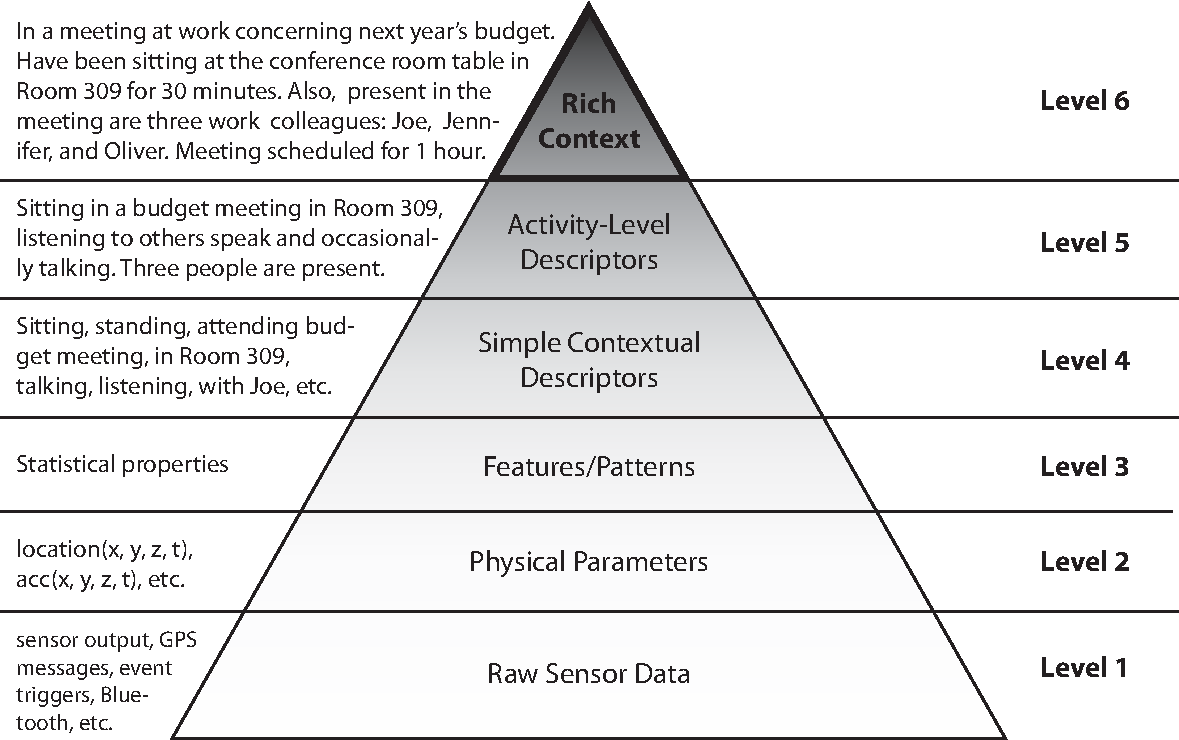
\includegraphics[width=1.0\textwidth]{Images/ContextPyramid4}
  \end{center}
  \caption[The Context Pyramid]{The ``context pyramid'' shows the different levels of processing to build context-aware systems, starting from raw sensor data at the bottom and working up to ``rich context'' at the highest level.}
  % Optional shorter caption in brackets is used in Table of Figures
  % (tof).
  \label{fig:context_pyramid}
\end{figure}
%

Lastly, we can make some general statements about how to process the input data in a context-sensing system. We conceptualize this process as a ``context pyramid'', which was first presented in [P3] and later in [P2]. This context pyramid is also shown in Figure~\ref{fig:context_pyramid} below. On the left side is an example of contextual information. At the bottom of the pyramid lies the raw input to the context-sensing system, such as sensor data. The difference between the first and second level in the pyramid is that in Level 2, some ``pre-processing'' of the data may have been performed, such as reference frame transformation or filtering out noise. In the next level of processing, statistical features are extracted from the data, such as mean values or frequency domain features computed from time series data. The distinction between ``pre-processing'' and statistical feature extraction can be a bit blurry in some cases, but generally speaking Level 2 data usually have a clear physical meaning, whereas Level 3 data might have only a mathematical or statistical meaning. Next, Level 4 is achieved after the Level 3 data is subjected to a function or algorithm that performs contextual classification or in some cases regression. This topic will be covered in greater detail in Chapter~\ref{ch:machine_learning}. Level 4 data is in the form of \emph{simple contextual descriptors}, which can be thought of as ``atomic'' elements of context. They each should belong to one of the seven categories described in Section~\ref{sec:framework} above. Then, Level 5 is achieved by combining multiple simple contextual descriptors into an activity-level description of the context, as well as the main pertinent contextual details. Finally, Level 6 combines all available contextual information into a \emph{rich context}. The aim at this level is to approach a description of the context that is indistinguishable from human-written prose. As was the case between Levels 2 and 3, the difference between Levels 5 and 6 can be sometimes blurry. In some context-aware systems there may be fewer processing steps or perhaps more, so even the number of levels should not be taken as dogma. We believe, however, that the general process will always follow the overall trend illustrated in the context pyramid.

This is true to a large extent even in the case of an ice-aware maritime route optimization system (i.e. Task 3), which appears at first sight very different from the example contextual information given in Figure~\ref{fig:context_pyramid}. At the bottom of the pyramid would lie raw data concerning the ice field, e.g.\ data from synthetic aperture radar (SAR) or other sources. The first step is to extract physical parameters from the raw data, such as a grid of values for ice thickness and ice concentration, or other system parameters such as the location of an ice breaker. Next, one might perform statistical analysis on the ice data, e.g.\ applying Gaussian process regression for the purposes of interpolation. Then, one uses features from Level 3 and a ship performance model, in order to estimate the ship's theoretical speed at coordinate $(lat, long)$. This is analogous to a Level 4 simple contextual descriptor (i.e. the \emph{in what manner} context). Next, the optimal route, computed from the Level 4 contextual information, is roughly analogous to an Activity-Level Descriptor at Level 5 because it is a higher-level context inferred from lower-level contextual information. Finally, combining the optimal route with other navigational information, such as weather information, maritime traffic information, etc., produces a rich contextual description describing the ship's current situation that approaches Level 6 at the top of the pyramid.
%
% \section{Conclusions}
% \label{sec:conclusions}
% %
% In this chapter we have defined the terms context and context awareness and provided a general introduction to the topic. We have attempted to discuss context awareness in an abstract and general way, but we have also pointed out the limitations of such a discussion. Our aim was to give a rough conceptual outline of this research topic, but our strong preference is that context should be discussed with some particular applications in mind, otherwise the subject is simply too broad to provide a general treatment. That being said, there are some general methods that can be employed towards many problems in context awareness, and such methods will be the focus of the next chapter.